\section{Modeling of the DC-Motor}

The purpose of this section is to establish a dynamic model of the DC-motor. This model will result in a transfer function from a voltage input, \textit{Um}, to an angular velocity output, \textit{$\omega_m$}. It will be done by modeling the electrical and the mechanical part of the motor and then putting them together to find the transfer function of the motor.

\subsection*{Electrical Model of the Motor}
The electrical circuit of the motor is presented in \autoref{fig:MotorCircuit}.

\begin{figure}[htbp]
	\centering
 	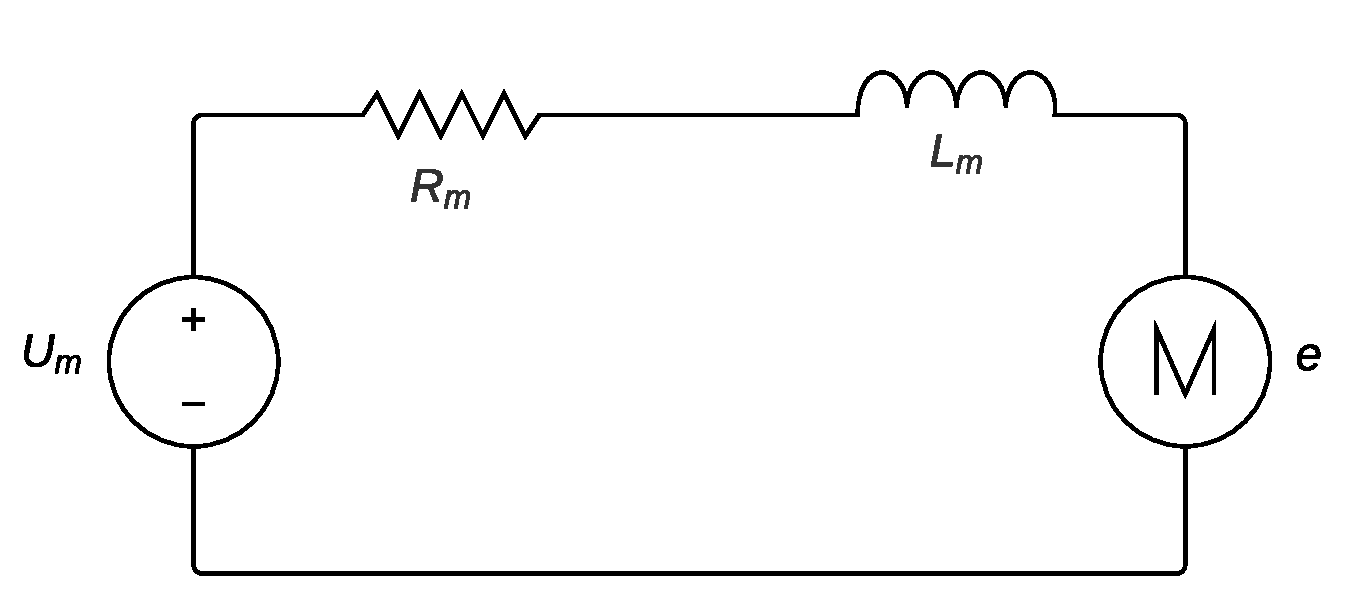
\includegraphics[width=0.7\textwidth]{figures/modeling/Motor/MotorElectricCircuit.pdf} 
 	\caption{Electric circuit of a DC-motor}
 	\label{fig:MotorCircuit}
\end{figure}

Using Kirchhoff's voltage law, the electric model of the DC-motor is found:
\begin{subequations} \label{eq:tech_ToA}
	\begin{flalign}
		&U_m = R_m \cdot i + L_m \frac{di}{dt} + e \addunit{\volt} \\
		&e = K_e \cdot \omega_m \addunit{\volt}
	\end{flalign}
\end{subequations}

\startexplain
	\explain{$U_m$ is the voltage output of the generator}{\si{\volt}}
	\explain{$R_m$ is the resistance of the DC-motor}{\si{\ohm}}
	\explain{$L_m$ is the inductance of the DC-motor}{\si{\henry}}
	\explain{$i$ is the current in the DC-motor}{\si{\ampere}}
	\explain{$e$ is the electromotive force}{\si{\volt}}
	\explain{$K_e$ is the motor velocity constant}{\si{\volt\second\per\radian}}
	\explain{$\omega_m$ is the angular velocity of the motor}{\si{\radian\per\second}}
\stopexplain

\subsection*{Mechanical Model of the Motor}
The mechanical circuit of the motor is presented in \autoref{fig:MotorBodyDiagram}.

\begin{figure}[htbp]
	\centering
 	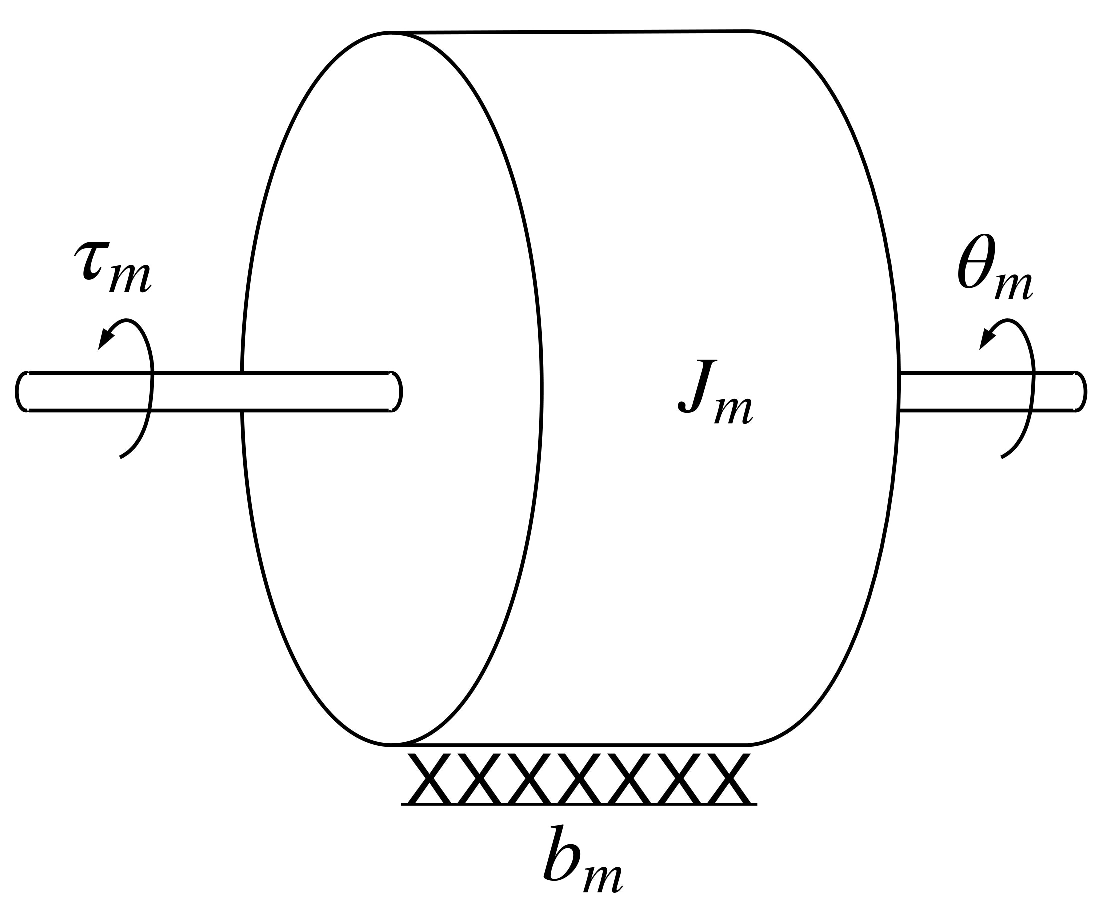
\includegraphics[width=0.4\textwidth]{figures/modeling/Motor/DCMotorMechanic.pdf} 
 	\caption{Body diagram of a DC-motor}
 	\label{fig:MotorBodyDiagram}
\end{figure}

When applied to a rotational movement, Newton's second law of motion state that the sum of the torques applied to an object equals the moment of inertia times the angular acceleration of this object. From \autoref{fig:MotorBodyDiagram}, the equation for the mechanical part of the motor is found:

\begin{equation}
	J_{m} \dot{\omega}_{m} = \tau_{m} - \tau_{l} - \tau_{fm} \addunit{\newton\meter}
	\label{eq:MotorMechanical}
\end{equation}

\startexplain
	\explain{$J_m$ is the moment of inertia of the motor}{\si{\kilo\gram\meter\squared}}
	\explain{$\omega_m$ is the angular velocity of the DC-motor}{\si{\radian\per\second}}
	\explain{$\tau_m$ is the torque of the DC-motor}{\si{\newton\meter}}
	\explain{$\tau_l$ is the torque of the load}{\si{\newton\meter}}
	\explain{$\tau_{fm}$ is the torque of the friction}{\si{\newton\meter}}
\stopexplain

The motor's torque and the friction's torque, respectively $\tau_m$ and $\tau_f$, are defined as:

\begin{subequations}\label{eq:tauLm}
	\begin{flalign}
		&\tau_m = K_t \cdot i \addunit{\newton\meter} \label{eq:MotorTorque}\\	
		&\tau_{fm} = b_{m}\cdot\omega_{m} \addunit{\newton\meter}	\label{eq:FrictionTorque}
	\end{flalign}
\end{subequations}

\startexplain
	\explain{$K_t$ is the motor torque constant}{\si{\newton\meter\per\ampere}}
	\explain{$b_m$ is the viscous friction coefficient}{\si{\newton\meter\second\per\radian}}
\stopexplain

Inserting \autoref{eq:tauLm} into \autoref{eq:MotorMechanical}:
\begin{equation}
	J_{m} \cdot \dot{\omega}_{m} = K_{t} \cdot i - \tau_{l} - b_{m} \cdot \omega_{m} \addunit{\newton\meter}
\end{equation}

\subsection*{Mechanical Model of the Motor}
First, both the electrical and the mechanical equations of the motor need to be Laplace-transformed:
\begin{subequations}
	\begin{flalign}
		&U_{m}(s) = R_{m} \cdot I(s) + s \cdot L_{m} \cdot I(s) + K_{e} \cdot \Omega_{m}(s) \addunit{1} \label{eq:ElectricalLaplace}\\	
		&s\cdot J_{m} \cdot \Omega_{m}(s) = K_{t} \cdot I(s) - \tau_{l} - B_{m} \cdot \Omega_{m}(s) \addunit{1}	\label{eq:MechanicalLaplace}
	\end{flalign}
\end{subequations}

The current, I(s), is isolated in \autoref{eq:ElectricalLaplace}:
\begin{equation}
	I(s)=\frac{U_m(s)-K_e\cdot\Omega(s)}{R_m+sL_m} \addunit{1}
	\label{eq:MotorCurrent}
\end{equation}

Then \autoref{eq:MotorCurrent} is inserted in \autoref{eq:MechanicalLaplace}:
\begin{equation}
	s\cdot J_{m} \cdot \Omega_{m}(s) = K_{t} \frac{U_m(s)-K_e\cdot\Omega_{m}(s)}{R_m+sL_m} - \tau_{l} - B_{m} \cdot \Omega_{m}(s) \addunit{1}
	\label{eq:Iinserted}	
\end{equation}

\autoref{eq:Iinserted} is simplified to find an expression for $\Omega_m$: 

\begin{subequations}
	\begin{flalign}
		&\Omega_m(s) \left(sJ_m + \frac{K_tK_e}{R_m + sL_m} + B_m \right) = \frac{K_tU_m(s) - \tau_l(R_m + sL_m)}{R_m + sL_m} \\	
		&\Omega_m(s) = \frac{K_tU_m(s) - \tau_l(R_m + sL_m)}{R_m + sL_m} \cdot \frac{R_m + sL_m}{sJ_m(R_m + sL_m) + B_m(R_m + sL_m) + K_tK_e} \\
		&\Omega_m(s) = \frac{K_tU_m(s) - \tau_l(R_m + sL_m)}{(J_mL_m)s^2 + (J_mR_m + B_mL_m)s + B_mR_m + K_tK_e} \addunit{1} \label{eq:DCMotorTFWithLoad}
	\end{flalign}
\end{subequations}
\autoref{eq:DCMotorTFWithLoad} is the transfer function of the DC-motor from a voltage $U_m(s)$ to an angular velocity $\omega_m$. This equation will be used for the rest of the modeling. 

\todo [inline, author=Geoff]{To be added in the DC-Motor Test appendix when it's created}
For the test of the DC-motor, there is no load. The torque of the load becomes zero, thus changing the expression of $\omega_m$: 
\begin{equation}\label{eq:Omega_m}
	\frac{\Omega_m(s)}{U_m(s)} = \frac{K_t}{(J_mL_m)s^2 + (J_mR_m + B_mL_m)s + B_mR_m + K_tK_e} \addunit{1}
\end{equation}









